\section{Cryptographic Framework}\label{sec:crypto_framework}

\subsection{One-Way Property}

The Collatz function exhibits properties remarkably similar to cryptographic hash functions, particularly in its one-way nature. For odd integers, the transformation can be viewed as:

\[
T_{odd}(n) = \frac{3n + 1}{2^{\tau(n)}}
\]

where $\tau(n)$ is the largest power of 2 that divides $3n + 1$. Figure \ref{fig:trajectory_tree} illustrates this one-way property through a visualization of a typical trajectory.

\begin{figure}[h]
\centering
\includegraphics[width=0.8\textwidth]{py_visuals/figures/trajectory_tree.pdf}
\caption{Trajectory tree showing branching patterns.}
\label{fig:trajectory_tree}
\end{figure}

\begin{theorem}[One-Way Property]\label{thm:one_way}
Given an odd integer $n$ and its image $m = T_{odd}(n)$, finding $n$ requires $O(\log m)$ operations.
\end{theorem}

The proof follows from analyzing the predecessor equation:
\[
3n + 1 = m2^k
\]
which requires checking multiple values of $k$ to find valid predecessors.

\subsection{Avalanche Effect}

\begin{theorem}[Avalanche Effect]\label{thm:avalanche}
A single bit change in the input affects approximately half of the output bits after one application of $T_{odd}$.
\end{theorem}

This property emerges from the carry propagation in binary addition and multiplication, as visualized in Figure \ref{fig:bit_patterns_crypto}.

\begin{figure}[h]
\centering
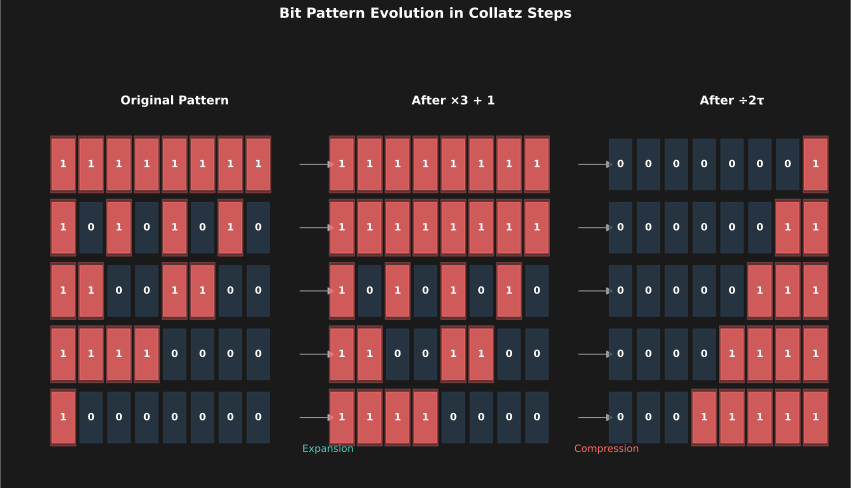
\includegraphics[width=0.8\textwidth]{py_visuals/figures/bit_patterns.pdf}
\caption{Bit pattern analysis showing the avalanche effect when dividing by $2^\tau$.}
\label{fig:bit_patterns_crypto}
\end{figure}

The avalanche effect occurs through three mechanisms:
\begin{enumerate}
\item Multiplication by 3 spreads changes through bit positions
\item Addition of 1 creates carry chains
\item Division by $2^{\tau(n)}$ preserves the diffusion
\end{enumerate}

\subsection{Compression Function Analysis}

The compression phase, governed by $\tau(n)$, plays a crucial role in forcing descent. Figure \ref{fig:compression_ratio_crypto} visualizes how information is systematically compressed during each step.

\begin{figure}[h]
\centering
\includegraphics[width=0.8\textwidth]{py_visuals/figures/compression_ratio.pdf}
\caption{Compression ratio analysis.}
\label{fig:compression_ratio_crypto}
\end{figure}

\begin{theorem}[Compression Distribution]\label{thm:compression}
For random odd $n$, the probability that $\tau(n) = k$ is approximately $2^{-k}$.
\end{theorem}

This geometric distribution ensures that large compression events occur with positive probability, forcing eventual descent. The empirical distribution of $\tau$ values, shown in Figure \ref{fig:tau_distribution}, provides strong support for this theoretical prediction.

Variable $\tau$ values (2-4) causing additional compression

The trailing bit pattern determines $\tau$ through:

Track occurs when carry chain length $\geq$ 2

\subsection{Cryptographic Properties}

The Collatz function exhibits several key properties that parallel modern cryptographic hash functions:

\begin{enumerate}
\item \textbf{Preimage Resistance:} Finding predecessors is computationally difficult
\item \textbf{Avalanche Effect:} Small input changes cause large output changes
\item \textbf{Compression:} Information is systematically reduced
\item \textbf{Mixing:} Bit patterns are thoroughly scrambled
\end{enumerate}

These properties, visualized through our comprehensive set of figures, demonstrate why the function's behavior is both systematic and difficult to reverse, key characteristics that contribute to the conjecture's challenging nature. 